\documentclass[11pt,a4paper,openany]{book} 

\usepackage{sasv}

\begin{document}

\pagenumbering{roman}

% ----------------------------------------------------------------------
% TITLE PAGE
% ----------------------------------------------------------------------
\begin{center}

{\btitle{TinyMLOps for Real-Time Keyword Spotting: Architecting an Automated, Resource-Constrained Deep Learning Pipeline on the Raspberry Pi Pico W}\vskip100pt}

\textbf{A Thesis Submitted}

\vskip5pt
In Partial Fulfillment of the Requirements 

\vskip5pt
for the Course of 

\vskip5pt
\textbf{Undergraduate Research}

\vskip5pt
\textit{by}

\vskip10pt
\textbf{Rishikesh Pandey}

\textbf{(PNR.: 220200051)}

\vskip50pt
% Make sure your university logo is saved as Logo.jpg in the Figures folder

\includegraphics{Figures/Logo.jpg}

\vfill
\vskip22pt
\textit{Submitted to the}

\vskip5pt
\textbf{School of Computing and Data Science}

\vskip5pt
\textbf{Sai University}

\vskip5pt
April 2026
\end{center}

\clearpage

% ----------------------------------------------------------------------
% CERTIFICATE PAGE
% ----------------------------------------------------------------------
% \begin{center}
% {\btitle{CERTIFICATE}\vskip16pt}
% \end{center}

% This is to certify that the work contained in the thesis entitled 
% ``\textbf{TinyMLOps for Real-Time Keyword Spotting: Architecting an Automated, Resource-Constrained Deep Learning Pipeline on the Raspberry Pi Pico W}'' by 
% \textbf{Rishikesh Pandey (PNR.: 220200051)} has been carried out under my 
% supervision. 

% \thispagestyle{empty}

% \vskip102pt
% \noindent
% {\begin{tabular*}{\linewidth}{@{\extracolsep{\fill}}ll@{\extracolsep{\fill}}}
% Date: \rule{3cm}{0.4pt} & \textbf{Dr. Ashok Chandrasekaran}\\
% &Assistant Professor\\
% &School of Computing and Data Science\\
% &Sai University, Chennai \\
% \end{tabular*}}

% \clearpage

% ----------------------------------------------------------------------
% ACKNOWLEDGEMENTS
% ----------------------------------------------------------------------
\chapter*{Acknowledgements}
\addcontentsline{toc}{chapter}{Acknowledgements}

I would like to express my profound gratitude to the Department of Computing and Data Science at Sai University for providing the flexibility to pursue this.

I am deeply indebted to my thesis supervisor, Dr. Ashok Chandrasekaran, for his invaluable guidance, patience, and constructive feedback throughout this project. His deep insights into machine learning and continuous encouragement pushed me to bridge the gap between theoretical data science and rigorous embedded engineering.

A special note of appreciation goes to the global open-source and TinyML communities. The implementation of this pipeline would not have been possible without the developers and maintainers of the Edge Impulse platform, the Raspberry Pi Foundation, and the creators of Data Version Control (DVC). Their commitment to democratizing edge intelligence heavily inspired the architectural decisions in this work.

I am also grateful to my friends and peers at Sai University, whose camaraderie, late-night debugging sessions, and collaborative spirit made this demanding journey incredibly rewarding.

\vspace{20pt}
\noindent
\textbf{Rishikesh Pandey}\\
Sai University\\
April 2026

\clearpage

% ----------------------------------------------------------------------
% ABSTRACT
% ----------------------------------------------------------------------
\chapter*{Abstract}
\addcontentsline{toc}{chapter}{Abstract}

The deployment of artificial intelligence to resource-constrained microcontrollers, known as TinyML, enables pervasive, real-time edge computing. However, transitioning a machine learning model from a cloud training environment to a physical embedded device introduces severe operational and architectural bottlenecks. Traditional manual deployment workflows are inherently unscalable, lack version control for heavy acoustic datasets, and frequently suffer from ``dependency hell'' during C++ firmware cross-compilation.

To resolve these challenges, this thesis proposes, architects, and validates a fully automated, end-to-end TinyMLOps pipeline for Real-Time Keyword Spotting (RT-KWS) on the Raspberry Pi Pico W. The proposed architecture bridges Data Engineering, Machine Learning, and DevOps. It utilizes Data Version Control (DVC) backed by AWS S3 to achieve hybrid, cryptographic traceability of acoustic datasets without bottlenecking the Source Code Management system. Continuous Integration and Continuous Deployment (CI/CD) orchestration is handled via GitHub Actions, which abstracts computational workloads to the Edge Impulse cloud API for Mel-Frequency Cepstral Coefficient (MFCC) feature extraction and 1-Dimensional Convolutional Neural Network (1D-CNN) training.

\vspace{15pt}
\noindent
\textbf{Keywords:} TinyMLOps; Keyword Spotting (KWS); Edge AI; Raspberry Pi Pico W; Continuous Deployment (CI/CD); Int8 Quantization; Model Compression; Convolutional Neural Networks (1D-CNN).

\clearpage

% ----------------------------------------------------------------------
% TABLE OF CONTENTS & LISTS
% ----------------------------------------------------------------------
\makeatletter
\def\@makeschapterhead#1{%
  \vspace*{50\p@}%
  {\parindent \z@ \raggedright
    \normalfont
    \interlinepenalty\@M
    \Huge \bfseries  #1\par\nobreak
    \vskip 40\p@
  }}
\makeatother

\tableofcontents\markboth{Contents}{Contents}

\listoffigures
\addcontentsline{toc}{chapter}{List of Figures}

\clearpage

\listoftables
\addcontentsline{toc}{chapter}{List of Tables}

% ----------------------------------------------------------------------
% MAIN CONTENT START
% ----------------------------------------------------------------------
%mainmatter
\clearpage
\pagenumbering{arabic}
% Chapter 1 will begin right here!
\chapter{Introduction}

\section{Background}

\subsection{The Evolution and Economic Limitations of Cloud-Centric Machine Learning}
Machine Learning (ML) has fundamentally redefined the boundaries of computational problem-solving. By leveraging vast neural network architectures, modern ML systems can extract complex patterns from high-dimensional data, achieving human-level performance in Natural Language Processing (NLP) and Computer Vision. However, the foundational architecture of this revolution has been overwhelmingly centralized. To achieve state of the art accuracy, Large Language Models (LLMs) and deep vision networks have scaled to billions of parameters, as initially catalyzed by the transformer architectures introduced by Vaswani et al. \cite{1}. Managing these monolithic architectures necessitated the birth of Machine Learning Operations (MLOps) - a specialized engineering discipline designed to automate the deployment, versioning, and monitoring of massive models across distributed cloud clusters.

However, despite the advancement of cloud MLOps, this centralized paradigm has hit a severe economic and infrastructural bottleneck. Operating massive ML models in the cloud requires staggering energy consumption, immense GPU clusters, and high-bandwidth continuous internet connectivity. From a consumer and enterprise perspective, this reliance on cloud inference is becoming economically unsustainable, particularly for continuous, ``always-on'' sensor applications.

This friction is highly visible in modern AI subscription models. For instance, querying state-of-the-art cloud models like Anthropic's Claude Opus 4.7 incurs high operational costs, with charging upwards of \$5 per million input tokens and \$15 per million output tokens \cite{2}. For applications requiring continuous real-time data streaming - such as analyzing 24/7 environmental audio for Keyword Spotting - transmitting this data to a cloud API would exhaust a user's monthly subscription privilege within hours. This token exhaustion frustrates consumers, drives churn, and ultimately impacts the revenue retention of major AI providers. As noted in foundational edge computing texts by Warden and Situnayake, the sheer cost of cloud compute and bandwidth is actively pushing organizations away from centralized AI for continuous monitoring tasks.

\subsection{The Birth and Gravity of Tiny Machine Learning (TinyML)}
To overcome the latency, privacy risks, and severe economic costs of cloud tokens, the industry mandate has shifted toward processing data exactly where it is generated: at the edge. Tiny Machine Learning (TinyML) emerged as the ultimate solution to this bottleneck. TinyML is the deployment of highly compressed machine learning models onto deeply embedded microcontrollers (MCUs) that operate on milliwatts of power and possess mere kilobytes of Static Random Access Memory (SRAM). By keeping data localized, TinyML tends to require zero cloud API tokens, operates with zero network latency, and ensures user data privacy.

The transition toward TinyML is not merely a niche academic pursuit; it is a macroeconomic shift that is currently disrupting the global hardware supply chain. The sheer scale and sensitivity of this paradigm shift were starkly demonstrated in March 2026 following the release of Google's ``TurboQuant'' - a highly aggressive memory-compression and quantization framework. Because TurboQuant proved that highly accurate AI models could run on vastly smaller memory footprints, major high-capacity storage manufacturers like Samsung and Micron experienced significant stock drops \cite{5}. As investors realized that the future of Edge AI did not inherently rely on expensive, high-capacity RAM chips, the industry recognized that the true value of AI had shifted from hardware capacity to algorithmic compression. The goal of modern ML is no longer just building bigger models, but utilizing advanced quantization to make AI lean enough to exist everywhere invisibly.

\subsection{The Operational Void: From TinyML to TinyMLOps}
The statistics underscoring this transition are extreme. A standard cloud MLOps pipeline manages models requiring gigabytes of RAM and containerized environments running on multi-gigahertz processors. In stark contrast, TinyML environments operate under severe constraints: the Raspberry Pi Pico W, a standard edge device, features an ARM Cortex-M0+ processor running at 133 MHz, with only 264 KB of SRAM and 2 MB of Flash storage \cite{7}.

While researchers have successfully developed algorithms to compress neural networks into these kilobytes, the operational deployment of these models remains fundamentally broken. The current state of TinyML development resembles the dark ages of software engineering: data is manually curated in silos, quantization scripts are executed by hand, and compiled binaries are physically flashed to microcontrollers via USB cables.

Deployment of TinyML models must be assessed in terms of memory footprint (RAM and Flash) and latency, as standardized by the MLPerf Tiny benchmark suite \cite{8}. Traditional cloud MLOps pipelines are entirely blind to these embedded hardware constraints. If an MLOps pipeline attempts to push a model that exceeds 264 KB to a Pico W, it will trigger a hard-fault memory overflow, essentially ``bricking'' the device.

This glaring operational void has necessitated the birth of TinyMLOps. TinyMLOps is the application of continuous integration and continuous deployment (CI/CD) specifically engineered for the physics of microcontrollers. It requires pipelines that not only test for statistical accuracy but automatically execute hardware-aware quantization, profile memory footprints ahead of time, and securely flash firmware over the air (OTA) to remote devices.

\subsection{Problem Statement}
Despite the urgent market demand for edge intelligence and the devastating economic costs of relying solely on cloud LLMs for continuous monitoring, highly automated operational frameworks for microcontrollers remain virtually non-existent. Even after rapid advancements in model compression techniques like quantization and pruning, very little has been done to automate the continuous lifecycle of these models from data curation to hardware deployment.

For example, an edge device without a CI/CD pipeline deployed in the field encounters ``data drift'' - such as a Keyword Spotting model failing due to a new type of background noise - the process to update that model is entirely manual, unscalable, and prone to catastrophic memory errors.

Therefore, this thesis addresses a critical infrastructural gap in modern Artificial Intelligence: the development, design, and implementation of a fully automated TinyMLOps pipeline for edge model deployment. Specifically, this work seeks to engineer an end-to-end framework capable of tracking acoustic data, automating cloud-based neural network training, enforcing strict microcontroller memory gates, and dynamically executing secure Over-The-Air (OTA) firmware updates for Real-Time Keyword Spotting on constrained embedded hardware.

\section{Motivation and Scope of the Research}

\subsection{Primary Intent and the Benchmark Application}
The primary intention driving this research is to systematically understand the operational bottlenecks that currently weakens embedded machine learning. As established in the problem statement, the AI industry possesses highly advanced compression algorithms, yet lacks the automated infrastructure to deploy them safely and continuously to remote hardware. To address this, this thesis proposes a formalized TinyMLOps architecture, inspired from the principle of traditional MLOps.

To rigorously validate this proposed architecture, Real-Time Keyword Spotting (RT-KWS) was selected as the prime implementation benchmark. KWS serves as the ultimate stress test for edge machine learning for several reasons. First, acoustic monitoring requires continuous, uninterrupted sensor sampling; streaming 24/7 audio to a cloud API is economically unfeasible due to rapid token exhaustion \cite{2} and introduces severe privacy liabilities. Second, processing 16 kHz audio requires complex, real-time Digital Signal Processing (DSP) to extract Mel-Frequency Cepstral Coefficients (MFCCs) before neural network inference can even begin. If an MLOps pipeline can successfully automate the training, compression, and Over-The-Air (OTA) deployment of a model as computationally demanding as RT-KWS on a strictly constrained microcontroller \cite{3}, the pipeline's architectural viability is unequivocally proven.

\subsection{Scope of the Research}
The scope of this thesis lies around the operational architecture and system-level integration of machine learning. Specifically, the scope encompasses:

\begin{description}
    \item[Developer-Side Automation:] The design of a deterministic data ingestion workflow utilizing Python-based audio segmentation and a hybrid storage architecture. This involves implementing Data Version Control (DVC) paired with AWS S3 to manage massive acoustic datasets, fully decoupled from the lightweight Git source code repository.
    \item[Continuous Integration (CI) and Optimization:] The engineering of a cloud-based CI factory using GitHub Actions. This pipeline automates API-driven model training, enforces statistical validation gates, and programmatically executes Int8 Post-Training Quantization (PTQ) and Ahead-of-Time (AOT) C++ compilation.
    \item[Deployment-Side Automation (CD):] The implementation of a secure, memory-safe OTA C++ update mechanism, allowing the Raspberry Pi Pico W to dynamically poll GitHub Releases and flash compiled binaries via Wi-Fi.
    \item[System-Level Analysis:] The empirical evaluation of the deployed models, tracking the exact impact of quantization and compiler optimization on Peak RAM usage, Flash (ROM) footprint, and millisecond classification latency.
\end{description}

\subsection{Academic and Industrial Significance}
The significance of this work lies in elevating the maturity of embedded machine learning from experimental prototyping to production-grade deployment. According to the MLOps maturity models defined by major cloud providers \cite{9}, the vast majority of current TinyML development exists at ``Level 0'' - characterized by manual, ad-hoc execution. This thesis significantly advances the field by providing a blueprint to achieve ``Level 2 MLOps'' specifically for microcontrollers.

\subsection{Practical Relevance in the Face of Data Drift}
In industrial IoT and consumer electronics, the operational environment is rarely static. The practical relevance of this thesis is most clearly demonstrated through the phenomenon of ``Data Drift.''

Consider a KWS system deployed in a smart home environment. The model may have been trained in a quiet laboratory and achieves 99\% accuracy. However, once deployed, the introduction of a new environmental sound - such as the hum of a newly installed air conditioning unit - alters the acoustic background profile. The KWS model's accuracy will silently degrade, yielding false positives or failing to recognize wake words.

Without an MLOps pipeline, updating this device requires a physical recall or manual USB flashing by a technician, which is practically impossible for millions of deployed consumer devices \cite{11}. The practical relevance of the proposed TinyMLOps architecture is that it completely solves this bottleneck. When data drift occurs, engineers simply append the new noise data to the AWS S3 dataset and push a single Git commit. The pipeline autonomously handles the rest: downloading the data, retraining the network to ignore the new noise, quantizing the weights, verifying the memory footprint, and silently patching the remote edge device via Wi-Fi.

\subsection{Expected Impact on the AI Ecosystem}
The expected impact of formalizing TinyMLOps is a massive democratization of Edge Intelligence. Currently, executing complex, automated AI deployments requires highly specialized, expensive hardware or deep reliance on cloud APIs. By proving that robust CI/CD pipelines can successfully deploy and manage deep neural networks on highly constrained, ultra-low-cost silicon (such as the Raspberry Pi Pico W), this work drastically lowers the barrier to entry for intelligent IoT.

Economically, this framework enables organizations to deploy ``always-on'' intelligence without incurring the crippling, recurring ``token tax'' associated with continuous cloud API polling \cite{2}. Furthermore, by automating the compression of these models, this architecture accelerates the hardware market shift.

\subsection{Extending Hardware Longevity and Sustainability}
A secondary, yet critical, motivation for this work is the mitigation of electronic waste (e-waste) and the promotion of hardware sustainability. Historically, as software and AI models grew more complex, older hardware was rendered obsolete and discarded because it lacked the memory or processing power to handle local computation.

The integration of automated quantization and AOT compilation within the TinyMLOps pipeline actively reverses this trend. By mathematically compressing deep learning models to fit within legacy or highly constrained memory boundaries, the operational lifespan of existing microcontroller infrastructure is vastly extended. Furthermore, the ability to continuously update the firmware of these devices over the air means that edge sensors can evolve and adapt to new tasks without requiring physical hardware replacement.

% Start of chapter 2
\chapter{Literature Review}

The transition of Machine Learning (ML) from centralized cloud servers to decentralized, constrained edge devices has catalyzed a massive body of academic and industrial research over the past few years. However, while algorithmic compression has matured rapidly, the operational frameworks required to manage these algorithms at scale remain fragmented. This chapter reviews the current state of the art literature across TinyML architectures, the foundational principles of MLOps, and the emerging paradigm of TinyMLOps to contextualize the necessity of the proposed automated deployment pipeline.

\section{The Paradigm Shift to TinyML and Hardware Constraints}

The foundational literature in this domain focuses on the limitations, growth, and evaluation metrics of running complex neural networks on microcontrollers (MCUs).

\vspace{1.5em}
\noindent\textbf{Paper Title:} \textit{TinyML: A Systematic Review and Synthesis of Existing Research} \cite{4}\\
\textbf{Journal Name:} 2022 International Conference on Artificial Intelligence in Information and Communication (ICAIIC)\\
\textbf{Year:} 2022\\
\textbf{Authors:} H. Han, J. Siebert

\vspace{0.5em}
\noindent\textbf{Key Inferences / Findings:}
\begin{itemize}
    \item This paper provides a comprehensive systematic review of the TinyML ecosystem by analyzing 47 academic publications, categorizing them into five elements: hardware, frameworks, datasets, use cases, and algorithms.
    \item The review identifies that Keyword Spotting (KWS) is the absolute dominant use case in the industry, representing 26.09\% of all TinyML deployments, followed by image classification and visual wake words.
    \item It highlights that TensorFlow Lite (TFLite) is the most widely adopted framework, but also notes that the severe constraints of Static Random Access Memory (SRAM) and Flash storage on hardware like the ARM Cortex-M series are the primary bottlenecks to deployment.
\end{itemize}

\vspace{0.5em}
\noindent\textbf{Relevance to this Thesis:} Han and Siebert's systematic review academically validates the core premise and scope of this thesis. By identifying Keyword Spotting as the dominant use case for TinyML, it justifies this project's selection of an RT-KWS application as the benchmark for testing the MLOps pipeline. Furthermore, the authors' identification of SRAM and Flash constraints as the ultimate bottleneck directly justifies this project's focus on integrating ``Peak RAM Usage'' and ``Flash Usage'' profiling into the CI/CD pipeline prior to deployment.

\vspace{2em}
\noindent\textbf{Paper Title:} \textit{Tiny Machine Learning (TinyML): Research trends and future application opportunities} \cite{13}\\
\textbf{Journal Name:} Array (Elsevier)\\
\textbf{Year:} 2026\\
\textbf{Authors:} H. Han, S. Trimi, S. M. Lee

\vspace{0.5em}
\noindent\textbf{Key Inferences / Findings:}
\begin{itemize}
    \item This bibliometric analysis maps the rapid, exponential growth of TinyML research (averaging a 59.23\% annual growth rate between 2020 and 2024), proving it is a rapidly maturing interdisciplinary field.
    \item The study emphasizes that TinyML is critical because it enhances data privacy, decreases latency, and minimizes power consumption by processing data locally, fundamentally bypassing the cloud.
    \item The authors identify several key future trajectories for the field, specifically highlighting the ``edge-to-cloud continuum'' - where computationally heavy tasks (like model training and optimization) occur in the cloud, while real-time inference is pushed to the edge device.
\end{itemize}

\vspace{0.5em}
\noindent\textbf{Relevance to this Thesis:} This paper provides the macroeconomic and structural justification for the architecture designed in this thesis. The ``edge-to-cloud continuum'' concept proposed by the authors is similar to what the GitHub Actions CI/CD pipeline implements. By utilizing the cloud to handle the heavy orchestration, training, and compilation of the neural network, and subsequently pushing only the optimized binary to the edge device for local execution, this thesis physically realizes the theoretical continuum advocated for by the authors.

\section{From MLOps to the Edge}

Before understanding TinyMLOps, it is crucial to understand the foundational principles of traditional Machine Learning Operations and why they fail when applied directly to edge devices.

\vspace{1.5em}
\noindent\textbf{Paper Title:} \textit{Machine Learning Operations (MLOps): Overview, Definition, and Architecture} \cite{14}\\
\textbf{Journal Name:} arXiv preprint arXiv:2205.02302\\
\textbf{Year:} 2022\\
\textbf{Authors:} D. Kreuzberger, N. Kühl, S. Hirschl

\vspace{0.5em}
\noindent\textbf{Key Inferences / Findings:}
\begin{itemize}
    \item The authors conduct a mixed-method research study to formally define MLOps, conceptualizing it as the intersection of machine learning, software engineering (DevOps), and data engineering.
    \item They identify nine foundational principles required for an MLOps pipeline: CI/CD automation, workflow orchestration, reproducibility, versioning (of data, model, and code), collaboration, continuous ML training, metadata tracking, continuous monitoring, and feedback loops.
    \item The research highlights that organizational silos and the lack of automated, reproducible workflows are the primary reasons why ML proofs of concept fail to reach production environments.
\end{itemize}

\vspace{0.5em}
\noindent\textbf{Relevance to this Thesis:} Kreuzberger et al. provide the similar software engineering blueprint used to construct the automation phases of this thesis. By formally defining the nine principles of MLOps, this paper guided the implementation of Data Version Control (DVC) to handle the ``versioning'' principle, and GitHub Actions to handle the ``CI/CD automation'' and ``workflow orchestration'' principles. However, while this paper perfectly defines cloud MLOps, it assumes the target deployment hardware consists of scalable cloud servers (e.g., Kubernetes clusters), leaving a gap for how to deploy to microcontrollers.

\vspace{2em}
\noindent\textbf{Paper Title:} \textit{TinyMLOps: Operational Challenges for Widespread Edge AI Adoption} \cite{15}\\
\textbf{Journal Name:} 2022 IEEE International Parallel and Distributed Processing Symposium Workshops (IPDPSW)\\
\textbf{Year:} 2022\\
\textbf{Authors:} S. Leroux, P. Simoens, M. Lootus, K. Thakore, A. Sharma

\vspace{0.5em}
\noindent\textbf{Key Inferences / Findings:}
\begin{itemize}
    \item This paper introduces the term ``TinyMLOps'' by arguing that moving from centralized cloud deployments to decentralized edge deployments introduces a host of new operational challenges.
    \item The authors highlight the ``Fragmented IoT Landscape,'' noting that deploying to the edge requires managing a massive variety of different vendors, architectures, and hardware capabilities, which breaks standard cloud containerization (like Docker).
    \item They argue that TinyMLOps platforms must automatically track different optimized versions (quantized, pruned) of a base model to target these different hardware constraints effectively.
\end{itemize}

\vspace{0.5em}
\noindent\textbf{Relevance to this Thesis:} Leroux et al. clearly define the same problem statement of this thesis. Traditional MLOps (as defined by Kreuzberger) fails at the edge because it cannot handle hardware fragmentation. This thesis directly answers the authors' call for a TinyMLOps platform by integrating hardware-aware optimizations. By utilizing the Edge Impulse APIs to automatically compile different versions of the model specifically for the ARM Cortex-M0+ architecture, this project solves the fragmentation challenge highlighted in this paper.

\section{Frameworks, Compilers, and Real-World Deployments}

The final domain of review focuses on the actual software frameworks and deployment mechanics required to operationalize the TinyMLOps loop.

\vspace{1.5em}
\noindent\textbf{Paper Title:} \textit{Edge Impulse: An MLOps Platform for Tiny Machine Learning} \cite{8}\\
\textbf{Journal Name:} Proceedings of the 6th MLSys Conference\\
\textbf{Year:} 2023\\
\textbf{Authors:} S. Hymel, C. Banbury, D. Situnayake, et al.

\vspace{0.5em}
\noindent\textbf{Key Inferences / Findings:}
\begin{itemize}
    \item This paper introduces Edge Impulse as a holistic MLOps platform specifically designed to solve the challenges of software fragmentation and hardware heterogeneity in TinyML.
    \item A critical technical finding is the superiority of Ahead-of-Time (AOT) compilation via the Edge Impulse ``EON Compiler.'' The authors prove that by compiling models directly to C++ source code - thereby removing the TensorFlow Lite for Microcontrollers (TFLM) interpreter overhead - Peak RAM and Flash usage are drastically reduced.
    \item The paper demonstrates the necessity of the ``EON Tuner'' (AutoML) to explore the complex co-optimization space between Digital Signal Processing (DSP) parameters and Neural Network configurations.
\end{itemize}

\vspace{0.5em}
\noindent\textbf{Relevance to this Thesis:} This paper is the technical backbone of the proposed pipeline's compilation stage. The empirical evidence provided by Hymel et al. regarding the memory efficiency of the EON Compiler serves as the justification for integrating it into the CI/CD workflow rather than relying on standard TFLM. By programmatically triggering the EON Compiler and DSP extraction blocks via the Edge Impulse API in the GitHub Actions runner, this thesis automates the same optimization techniques proven effective in this MLSys paper.

\vspace{2em}
\noindent\textbf{Paper Title:} \textit{A TinyMLOps Framework for Real-world Applications} \cite{11}\\
\textbf{Journal Name:} River Publishers Series (Book Chapter 12)\\
\textbf{Year:} 2024\\
\textbf{Authors:} M. Antonini, M. Vecchio, F. Antonelli

\vspace{0.5em}
\noindent\textbf{Key Inferences / Findings:}
\begin{itemize}
    \item The authors propose a comprehensive TinyMLOps loop consisting of specific phases: Plan, Create, Adapt \& Optimize, Verify, Package, Release, Configure, and Monitor.
    \item A major contribution is the proposed architecture utilizing tools like MLFlow for experiment tracking and MicroPython as a Hardware Abstraction Layer (HAL).
    \item The paper notes a severe limitation in standard embedded deployment: models hardcoded into C/C++ firmware require a complete Over-The-Air (OTA) flash of the entire device memory to be updated, which is risky and inflexible compared to deploying simple Python scripts.
\end{itemize}

\vspace{0.5em}
\noindent\textbf{Relevance to this Thesis:} This paper outlines the exact operational loop that this thesis automates. The 8-step TinyMLOps loop defined by Antonini et al. is physically realized by the GitHub Actions pipeline. Furthermore, the authors' warning regarding the dangers of hardcoded firmware OTA updates directly informs the ``Future Scope'' section of this thesis. While this project successfully implemented C++ chunked OTA flashing, the risks identified in this paper serve as the primary justification for proposing Dual-Bank (A/B) flash partitioning for future enterprise-grade deployments.

% Chapter 3 will begin right here!
\chapter{Methodology and Implementation Details}

The transition from a traditional, manual embedded development workflow to an automated Machine Learning Operations (MLOps) paradigm requires a robust design of the system architecture. The proposed TinyMLOps framework is a closed-loop, fully automated deployment architecture engineered specifically for the resource-constrained Raspberry Pi Pico W. Its primary objective is to eliminate the friction between heavy acoustic data curation, cloud-based neural network training, and the physical constraints of microcontroller deployment.

\section{Broad Tiny MLOps System Architecture}

\begin{figure}[!ht]
    \centering
    % Ensure you save the downloaded Google architecture image in your Figures folder as 'General_MLOps.jpg'
    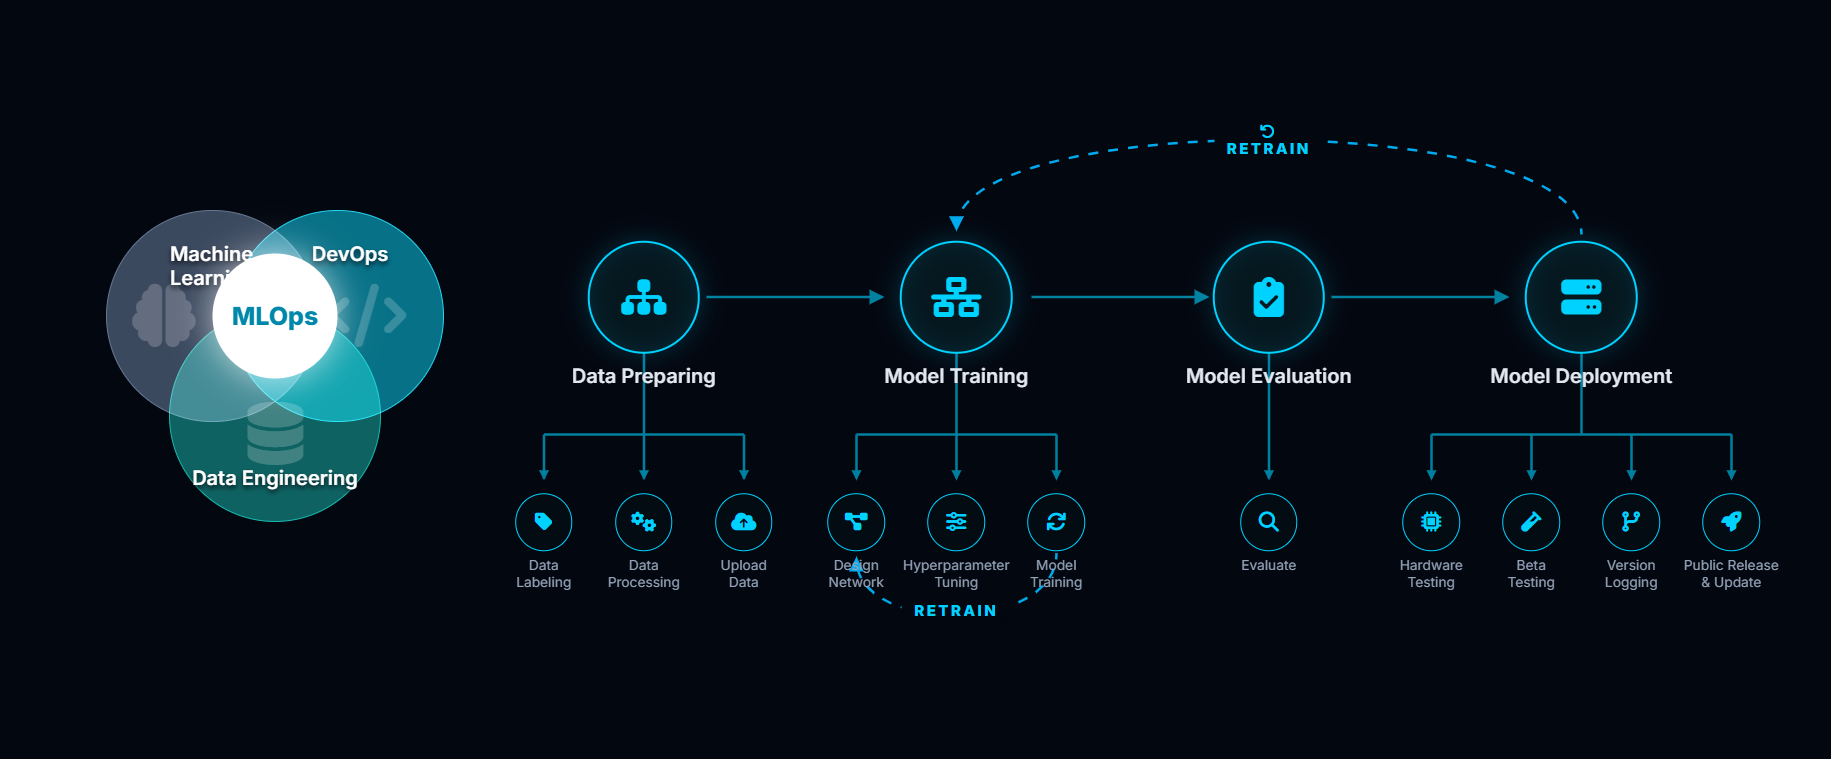
\includegraphics[width=\linewidth]{Figures/General_MLOps.jpg}
    \caption{General MLOps Architecture}% credit: Google, https://www.geminiopencloud.com/en/solutions/ml-devops/}
    \label{fig:general_mlops}
\end{figure}
Image credit: Google, https://www.geminiopencloud.com/en/solutions/ml-devops/

Deploying artificial intelligence on deeply embedded, resource-constrained microcontrollers demands a formalized, automated operational framework. The TinyMLOps architecture provides a closed-loop lifecycle, systematically transforming raw sensor data into an optimized, executable hardware binary. This Architecture is the blend of DevOps, ML, and MLOps. This architecture is widely used. We use this as the parent architecture for our specialized use case of a KWS application. 

\subsection{The Convergence of Disciplines}
TinyMLOps operates at the intersection of three computer science domains:
\begin{itemize}
    \item \textbf{Data Engineering:} Manages the ingestion, sanitization, and cryptographic versioning of high-velocity, heterogeneous sensor data within cloud-based storage.
    \item \textbf{Machine Learning:} Governs the theoretical design of neural network topologies, hyperparameter tuning, and feature extraction mathematics.
    \item \textbf{DevOps (Software Engineering):} Provides the CI/CD infrastructure for automated testing, hardware-aware compiler execution, and secure Over-The-Air (OTA) firmware provisioning.
\end{itemize}

\subsection{The 4-Stage Pipeline}
\begin{description}
    \item[Stage 1: Data Preparation] Acts as a deterministic filter for constrained devices. Raw data undergoes rigorous cleaning and formatting before being uploaded to centralized, content-addressable storage for immutable version control.
    \item[Stage 2: Model Training \& Optimization] Executed within a scalable cloud factory. Automated Machine Learning (AutoML) sweeps through hyperparameter combinations. An internal Retrain Loop iteratively adjusts the network topology until the training loss converges to a mathematical global minimum.
    \item[Stage 3: Model Evaluation (Quality Gate)] The model is profiled against the ``Iron Triangle'' of TinyML: Generalization Accuracy, Peak RAM, and Flash ROM footprint. Compression techniques (e.g., Post-Training Quantization) shrink the payload. If the compiled binary exceeds the target microcontroller's physical memory limits, deployment is violently halted to prevent hardware overflows.
    \item[Stage 4: Deployment \& Operations] The optimized model is compiled to raw C/C++ or packaged with a lightweight interpreter. This model then goes through rigorous testing in multiple stages. If it passes through all the testing stages, it is securely released. This operates as a localized inference engine completely decoupled from the cloud. The device periodically transmits lightweight health and predictive confidence telemetry.
\end{description}

\subsection{The Continuous Feedback Loop (Data Drift)}
A mature MLOps pipeline is non-linear. A macro-level RETRAIN path continuously links deployment back to training. If environmental conditions shift (e.g., a new background noise is introduced), the model experiences Data Drift and its accuracy silently decays. The on-device monitoring component detects this drop in predictive confidence and autonomously triggers the retraining pipeline - ingesting new data, retraining a more robust model, and deploying an updated firmware patch.

\section{Implementation of the Tiny MLOps for Keyword Spotting Application}

\subsection{Local Data Preparation and Hybrid Version Control}
The execution of the Real-Time Keyword Spotting (RT-KWS) TinyMLOps pipeline begins within the localized Developer-Side Infrastructure. Before any machine learning or cloud orchestration can occur, the raw acoustic environment must be curated, standardized, and strictly version-controlled. This initial phase isolates the heavy data-wrangling tasks to the local environment, ensuring that only sanitized data and lightweight code pointers are eventually pushed to the cloud integration servers.

\subsubsection{Acoustic Data Curation and Standardization}
The foundation of the KWS model is the raw acoustic dataset. However, raw environmental audio is inherently unstructured, varying wildly in sampling rates, bit depths, channel counts, and temporal lengths. Because the downstream target hardware (the Raspberry Pi Pico W) and the Edge Impulse DSP pipeline expect a deterministic input tensor, the dataset must be forced through a strict sanitization protocol. The dataset for this project has been taken from Google's speech command dataset, and a self-curated one.

To achieve this, a custom Python-based sanitization algorithm (conceptually defined as \texttt{chopper.py}), utilizing the \texttt{pydub} and \texttt{librosa} audio processing libraries, is executed locally. We do three things:

\begin{enumerate}
    \item \textbf{Nyquist-Compliant Resampling:} Human speech phonemes essential for keyword recognition generally fall below 8 kHz. To satisfy the Nyquist-Shannon sampling theorem without wasting subsequent memory on ultrasonic frequencies, the script down-samples all audio files to exactly 16 KHz. The audio is simultaneously down-mixed to a single (mono) channel with a 16-bit Pulse-Code Modulation (PCM) depth.
    \item \textbf{Deterministic Temporal Slicing:} The algorithm utilizes a sliding window to parse continuous audio streams, slicing them into exact 1-second arrays. Any trailing audio frames that fail to meet this 1-second threshold are discarded to prevent the introduction of zero-padding artifacts. This guarantees that every sample uploaded to the cloud will contain an identical $16,000 \times 1$ raw amplitude array.
    \item \textbf{Class Merging and Directory Structuring:} To optimize the model's decision boundaries for real-world inference, the sliced audio is sorted into three terminal classification directories: \textit{yes}, \textit{no}, and \textit{noise}. Ambient silence, unpredictable static, and non-target speech are mathematically merged into the \textit{noise} class. This proactive curation drastically reduces false-positive wake words when the Pico W is later exposed to noisy environments.
\end{enumerate}

\subsubsection{Hybrid Version Control via DVC and AWS S3}
Once the acoustic data is sanitized, it must be versioned alongside the deployment source code. A foundational principle of the MLOps paradigm is the strict versioning of data, code, and models to ensure complete reproducibility and traceability. However, traditional Source Code Management (SCM) systems, such as Git, are architected to track line-by-line differential changes in plain text. When tasked with tracking thousands of binary \texttt{.wav} files, Git attempts to compress and store the entire binary payload for every modification. This rapidly inflates the \texttt{.git} directory, severely bottlenecking repository cloning and causing continuous integration (CI) pipelines to crash.

To bypass this structural limitation, the proposed architecture implements a hybrid storage methodology utilizing Data Version Control (DVC) backed by an Amazon Web Services (AWS) S3 bucket. DVC operates as a content-addressable storage manager directly integrated into the Git workflow.

Instead of committing the heavy acoustic binaries to Git, DVC mathematically computes a unique MD5 cryptographic hash for each 1-second \texttt{.wav} file based entirely on its binary contents. DVC physically moves the heavy audio files to the AWS S3 remote storage bucket under their respective hash directories. It then generates microscopic, plaintext pointer files (e.g., \texttt{dataset.dvc}) that contain only the MD5 hashes and file sizes.

Only these lightweight \texttt{.dvc} pointer files, alongside the C++ deployment logic and GitHub Actions YAML scripts, are committed to the GitHub repository. This effectively decouples the heavy dataset from the SCM while maintaining an immutable, cryptographic link between the exact state of the acoustic data and the specific version of the source code. This hybrid architecture ensures that the repository remains agile and ready for Phase 2: CI/CD Orchestration, where the cloud factory will utilize these pointers to reconstruct the exact training environment.
% 3.3
\section{CI/CD Orchestration and Cloud-Based Neural Network Training}

With the local acoustic data perfectly curated, segmented, and securely hashed via DVC, the TinyMLOps pipeline transitions from the developer's local environment to the cloud. This transition strictly enforces the foundational MLOps principles of continuous integration, automated workflow orchestration, and strict reproducibility. The heavy computational lifting is completely abstracted away from the local machine and handed over to an automated pipeline orchestrated by GitHub Actions and the Edge Impulse cloud infrastructure.

\subsection{GitHub Actions and the Ingestion API Pipeline}
To eliminate structural bottlenecks caused by manual execution, the pipeline utilizes GitHub Actions as the primary orchestration engine. The automation sequence is triggered the moment a developer commits an updated \texttt{.dvc} pointer file or deployment script to the main repository branch.

Upon triggering, an ephemeral Ubuntu runner is provisioned in the cloud and executes a predefined YAML workflow:

\begin{itemize}
    \item \textbf{Building Docker:} The GitHub Actions runner spins up a Docker container based on your dockerfile, and rest all the actual compilation scripts run entirely inside that Docker container's isolated environment.
    \item \textbf{Data Retrieval:} The runner authenticates with Amazon Web Services (AWS) using securely injected repository secrets. It executes the \texttt{dvc pull} command, which reads the committed MD5 hashes, queries the AWS S3 bucket, and downloads the exact binary \texttt{.wav} files required to perfectly replicate the acoustic dataset.
    \item \textbf{API Orchestration:} Rather than training the model locally on the GitHub runner, the pipeline leverages the Edge Impulse REST API. The runner utilizes Python request libraries to securely push the downloaded acoustic dataset into the Edge Impulse backend.
    \item \textbf{Triggering the DSP Pipeline:} Once the data is ingested, the GitHub runner triggers the Edge Impulse cloud factory to execute the Mel-Frequency Cepstral Coefficient (MFCC) mathematical transformations (as explicitly defined in Section 3.2.2). This generates the 2-Dimensional spectrograms necessary for neural network training.
\end{itemize}

\subsection{Mathematical Formulation of Feature Extraction (MFCC)}
Feeding 16,000 raw amplitude values directly into a dense neural network is computationally unviable for the Pico W. To achieve the necessary dimensionality reduction, the pipeline applies Mel-Frequency Cepstral Coefficients (MFCCs). The MFCC pipeline acts as a mathematical model of the human cochlea, isolating the phonetic characteristics of human speech while discarding background harmonic noise.

The extraction pipeline processes the 1-second audio array through a rigorous five-step mathematical sequence:

\paragraph{1. Pre-Emphasis Filtering}
The raw audio signal $x[n]$ inherently possesses higher energy at lower frequencies than at higher frequencies. To balance the frequency spectrum and improve the Signal-to-Noise Ratio (SNR), a first-order high-pass filter is applied to amplify the high-frequency acoustic energies. This is represented by the difference equation:
\begin{equation}
y[n] = x[n] - \alpha x[n-1]
\end{equation}
where $\alpha$ is the pre-emphasis coefficient, optimally set to $0.98$ for speech recognition tasks within this pipeline.

\paragraph{2. Framing and Windowing}
Audio is a non-stationary signal, meaning its statistical frequencies change over time. To process it, the signal is partitioned into short, overlapping temporal frames (Window Size = 20 ms, Stride = 20 ms). However, artificially slicing a continuous wave creates abrupt amplitude drops at the edges of the frames, causing high-frequency artifacts known as spectral leakage. To counteract this, a Hamming window is applied to each frame, tapering the edges to zero:
\begin{equation}
w[n] = 0.54 - 0.46 \cos\left(\frac{2\pi n}{N-1}\right)
\end{equation}
where $N$ is the number of samples per frame.

\paragraph{3. Fast Fourier Transform (FFT) and Power Spectrum}
The time-domain frames are then converted into the frequency domain to identify the constituent pitches. This is achieved using an $N$-point Fast Fourier Transform (FFT):
\begin{equation}
X[k] = \sum_{n=0}^{N-1} x[n] e^{-j \frac{2\pi k n}{N}}
\end{equation}
The periodogram estimate of the power spectrum is then calculated to determine the energy magnitude present at each frequency:
\begin{equation}
P[k] = \frac{1}{N} |X[k]|^2
\end{equation}

\paragraph{4. Mel Filterbank Application}
Human hearing does not perceive pitch linearly; the human ear is far more capable of distinguishing between low frequencies than high frequencies. To mimic this non-linear perception, the power spectrum is mapped onto the Mel scale using a bank of 32 overlapping triangular filters. The mathematical conversion from standard frequency ($f$ in Hertz) to the Mel scale ($m$) is defined as:
\begin{equation}
m = 2595 \log_{10}\left(1 + \frac{f}{700}\right)
\end{equation}
Applying these filters smooths the spectrum and highlights the specific frequency bands most critical to human voice recognition.

\paragraph{5. Discrete Cosine Transform (DCT)}
Because the Mel filterbanks are highly overlapping, the resulting filterbank energies are highly correlated. To decorrelate these features for the neural network, the logarithm of the filterbank energies is taken, and a Discrete Cosine Transform (DCT) is applied:
\begin{equation}
C[m] = \sum_{k=1}^{K} \log(E_k) \cos\left[m \left(k - 0.5\right) \frac{\pi}{K}\right]
\end{equation}
where $E_k$ represents the energy of the $k$-th Mel filter, and $K$ is the total number of filters (32).

The DCT physically compresses the spectral envelope into a sequence of coefficients. By retaining only the first 13 coefficients per frame - and deliberately discarding the higher-order coefficients that represent rapid, noisy spectral changes - the raw audio is successfully compressed. 

The below table mentions the information regarding the MFCC parameters:

\vspace{1em}

\begin{table}[!ht]
\centering
\caption{Time Series and MFCC Parameters}
\label{tab:mfcc_params}
\renewcommand{\arraystretch}{1.3} 
\begin{tabular}{|l|l|p{7.5cm}|}
\hline
\textbf{Parameter} & \textbf{Value} & \textbf{Description} \\ \hline
Window Size & 1000 ms & The length of the audio sample processed at once. \\ \hline
Window Increase (Stride) & 500 ms & The overlap between processing windows. \\ \hline
Frequency & 16000 Hz & Standard sampling rate for voice recognition. \\ \hline
MFCC Coefficients & 13 & Number of features extracted per frame. \\ \hline
Frame Length & 0.02 & Length of the FFT window. \\ \hline
Filter Number & 32 & Number of Mel filters applied. \\ \hline
DSP Processing Time & 154 ms & Latency to extract features on target hardware. \\ \hline
DSP Peak RAM & 15 KB & Memory required for feature extraction. \\ \hline
\end{tabular}
\end{table}

\FloatBarrier


\paragraph{Conclusion of the DSP Phase}
Through this sequential mathematical transformation, the initial $16,000 \times 1$ raw audio array is compressed into a 2-Dimensional spectrogram matrix. When flattened, this yields exactly 650 optimized features. This massive dimensionality reduction is the fundamental enabler of the TinyMLOps pipeline, allowing the subsequent 1D-CNN to execute within the strict 264 KB SRAM limit of the Raspberry Pi Pico W.

\subsection{The 1-Dimensional Convolutional Neural Network (1D-CNN) Topology}
Because the MFCC extraction phase formats the acoustic data into a spatial representation (frequency energies over time), the Edge Impulse backend dynamically constructs a 1-Dimensional Convolutional Neural Network (1D-CNN). 1D-CNNs are exceptionally efficient for sequential time-series data on microcontrollers, providing high accuracy without the massive parameter overhead of recurrent architectures.

The network topology executes sequentially through the layers described in the table below:

\vspace{1em}

\begin{table}[!ht]
\centering
\caption{1D-CNN Architecture Details}
\label{tab:1dcnn_arch}
\renewcommand{\arraystretch}{1.3} 
\begin{tabular}{|l|l|p{6.5cm}|}
\hline
\textbf{Layer Name} & \textbf{Configuration / Output Shape} & \textbf{Activation / Purpose} \\ \hline
Input Layer & 650 features & Receives the flattened MFCC spectrogram. \\ \hline
Reshape Layer & 13 columns & Formats data for 1D convolution. \\ \hline
1D Conv / Pool & 16 filters, 3 kernel size & Extracts initial audio patterns. \\ \hline
Dropout & Rate: 0.25 & Regularization to prevent overfitting. \\ \hline
1D Conv / Pool & 32 filters, 3 kernel size & Extracts deep, complex audio patterns. \\ \hline
Dropout & Rate: 0.25 & Further regularization. \\ \hline
Flatten Layer & N/A & Converts 2D feature maps to a 1D vector. \\ \hline
Dense Layer & 128 neurons & Fully connected classification layer. \\ \hline
Output Layer & 3 Classes (no, noise, yes) & Softmax layer for final probability output. \\ \hline
\end{tabular}
\end{table}

\FloatBarrier

\noindent \textbf{Training Hyperparameters:}
\begin{itemize}
    \item \textbf{Epochs (Training Cycles):} 10
    \item \textbf{Learning Rate:} 0.005
    \item \textbf{Batch Size:} 32
    \item \textbf{Validation Split:} 20\%
\end{itemize}

\section{Neural Network Training, Optimization, and Quality Gates}
Following the successful generation of the MFCC spectrograms via the Edge Impulse ingestion API, the TinyMLOps pipeline initiates the core machine learning phase. Because the acoustic data has been perfectly framed and transformed into a 2-Dimensional spatial representation of frequency energies over time, the cloud factory dynamically provisions a 1-Dimensional Convolutional Neural Network (1D-CNN) to perform the classification.

\subsection{The 1D-CNN Topology}
Standard 2D-CNNs (commonly used for image processing) and Recurrent Neural Networks (RNNs) require millions of parameters, drastically exceeding the 264 KB SRAM constraint of the Raspberry Pi Pico W. A 1D-CNN is selected because it is mathematically optimized for temporal, time-series data. It aggressively shares weights across the temporal dimension, drastically reducing the parameter count while maintaining the ability to detect distinct phonetic transitions.

The network topology executes sequentially through the following mathematical layers:

\paragraph{Input and Reshape Layer}
The flattened array of 650 MFCC features is ingested from the DSP phase and mathematically reshaped into a tensor matrix of $13 \times 50$, representing the 13 distinct Mel-frequency coefficients distributed across 50 discrete temporal frames (the 1-second audio window).

\paragraph{1D Convolutional Layer}
A 1D convolutional kernel (filter) slides exclusively across the temporal axis of the MFCC matrix to detect localized acoustic patterns. The discrete 1D convolution of the input sequence $f$ and the trainable kernel $g$ of size $M$ is defined as:
\begin{equation}
(f * g)[n] = \sum_{m=0}^{M-1} f[m] \cdot g[n - m]
\end{equation}
The network deploys multiple parallel filters (typically 8 to 16 channels) to extract hierarchical abstractions, such as pitch contours and plosive transients. The output tensor is then passed through a Rectified Linear Unit (ReLU) activation function, defined as $f(x) = \max(0, x)$. ReLU introduces the non-linearity necessary to learn complex vocal boundaries while remaining computationally trivial for the Pico W's Arithmetic Logic Unit (ALU).

\paragraph{Dropout Regularization}
Neural networks trained on constrained, localized acoustic datasets are highly susceptible to overfitting - memorizing the exact background noise of the training data rather than generalizing the phonetic wake-word. To prevent this, a Dropout layer is injected during the cloud training loop. The Dropout layer acts as a stochastic regularizer, randomly zeroing out a fraction $p$ of the incoming neurons during each training epoch. For a given neuron activation $h_i$, its output $y_i$ becomes:
\begin{equation}
y_i = \begin{cases} 
      \frac{h_i}{1-p} & \text{with probability } 1-p \\ 
      0 & \text{with probability } p 
   \end{cases}
\end{equation}
By scaling the active neurons by $\frac{1}{1-p}$, the expected mathematical sum of the activations remains constant. This forces the network to learn redundant, distributed pathways for recognizing the keyword, vastly increasing its real-world robustness against unseen voices.

\paragraph{Fully Connected (Dense) and Softmax Classification}
The abstracted spatial features are flattened into a 1D vector and passed into a fully connected dense layer. The terminal layer consists of exactly 3 output neurons, corresponding to the target classes established during local data curation: \textit{yes}, \textit{no}, and \textit{noise}. The network applies the Softmax function to convert the raw logits ($z_i$) into a normalized probability distribution ($P_i$) bounded between 0 and 1:
\begin{equation}
P_i = \frac{e^{z_i}}{\sum_{j=1}^{C} e^{z_j}}
\end{equation}
where $C$ represents the total number of classes.

\subsection{Int8 Post-Training Quantization (PTQ) and Automated Quality Gates}
A neural network trained in the cloud defaults to a 32-bit floating-point (Float32) representation. Deploying a Float32 model to an MCU lacks hardware efficiency; it consumes excessive SRAM, inflates the flash binary, and severely bottlenecks inference latency due to the lack of a dedicated floating-point unit (FPU) on many edge processors.

Before the Edge Impulse platform completes its workflow, it applies Int8 Post-Training Quantization (PTQ). PTQ acts as a lossy mathematical compression algorithm. It maps the continuous, 32-bit floating-point weights and activations ($R$) of the trained network to an 8-bit discrete integer grid ($Q$) ranging from -128 to 127. This mapping is achieved using a calculated scale factor ($S$) and a zero-point offset ($Z$):
\begin{equation}
Q = \text{round}\left(\frac{R}{S}\right) + Z
\end{equation}
This transformation shrinks the physical memory footprint by nearly 75\% and leverages the ARM Cortex-M0+ integer instruction sets to radically accelerate inference speeds, all while sacrificing less than a fraction of a percent in model accuracy.

\paragraph{The Automated Quality Gate (SIL Testing)}
Immediately following quantization, the pipeline executes its final cloud-side directive: the Automated Quality Gate. The Edge Impulse infrastructure runs a Software-in-the-Loop (SIL) evaluation against an unseen, holdout dataset. The pipeline strictly profiles the model against the ``Iron Triangle'' of TinyML:
\begin{itemize}
    \item \textbf{Generalization Accuracy:} Must exceed the predefined confidence threshold.
    \item \textbf{Peak RAM Consumption:} Must not exceed the Pico W's available dynamic memory.
    \item \textbf{Flash ROM Footprint:} Must fit within the defined firmware partition.
\end{itemize}

If the quantized model fails any of these three metrics, the Edge Impulse API returns a fatal error code to the GitHub Actions runner. The pipeline violently halts, deliberately failing the CI/CD build to prevent a degraded or hardware-overflowing model from reaching the C++ compilation phase.

\section{Target Compilation and Automated Release (Continuous Deployment)}

Once the Int8 quantized model successfully clears the automated Software-in-the-Loop (SIL) quality gates within the cloud factory, the TinyMLOps pipeline enters its final phase: Continuous Deployment (CD). This phase bridges the gap between high-level machine learning mathematics and bare-metal microcontroller execution. The pipeline must autonomously strip away all cloud-based abstraction, generate hardware-specific C++ instructions, and compile the final firmware executable without human intervention.

\subsection{Ahead-of-Time (AOT) Compilation via the EON\texttrademark{} Compiler}
Standard deployment methodologies for edge ML rely on interpreters (such as TensorFlow Lite for Microcontrollers). Interpreters require the MCU to load the neural network schema into RAM at runtime and dynamically resolve operations layer-by-layer. While flexible, this interpreter overhead consumes vital SRAM and introduces significant inference latency, which is detrimental to Real-Time Keyword Spotting on the 264 KB Raspberry Pi Pico W.

To eliminate this bottleneck, the pipeline utilizes Edge Impulse's EON (Edge Optimized Neural) Compiler to perform Ahead-of-Time (AOT) compilation. Instead of exporting a \texttt{.tflite} model graph, the EON compiler translates the neural network topology directly into heavily optimized, raw C++ source code.

By hardcoding the network operations and statically allocating memory buffers at compile-time, the EON compiler completely removes the interpreter payload. This architectural optimization yields up to a 40\% reduction in peak RAM usage and drastically accelerates inference execution by natively leveraging the ARM Cortex-M0+ DSP instruction set. The Edge Impulse API autonomously packages this generated C++ library and transmits it back to the waiting GitHub Actions runner.

\subsection{Automated Firmware Integration and CMake Build}
Upon receiving the optimized C++ ML library, the GitHub Actions runner transitions from a data orchestrator to a remote build server. The runner executes a predefined sequence to integrate the newly generated intelligence with the target hardware's operational logic:

\begin{itemize}
    \item \textbf{Source Code Merging:} The runner automatically merges the downloaded ML library with the primary RT-KWS application code residing in the GitHub repository. This application code handles the physical hardware peripherals, including the configuration of the Direct Memory Access (DMA) and the Inter-IC Sound (I2S) protocols required to continuously sample the Pico W's microphone at 16 kHz.
    \item \textbf{Cross-Compilation via CMake:} The ephemeral Ubuntu runner initializes the official Raspberry Pi Pico SDK toolchain. Using CMake, it cross-compiles the merged C++ source code specifically for the RP2040 dual-core architecture.
    \item \textbf{Binary Generation:} The compiler links the libraries and generates the final, executable \texttt{.bin} (USB Flashing Format) binaries. If a syntax error, memory overflow, or linking failure occurs during this phase, the CI/CD pipeline throws a fatal exception, immediately halting the deployment and alerting the development team.
\end{itemize}

\subsection{Cryptographic Versioning and Public Release}
The successful compilation of the \texttt{.bin} binary represents the culmination of the TinyMLOps sequence. However, a core tenet of MLOps is strict traceability - an isolated binary is useless in a production environment if its lineage is unknown.

Before deployment, the GitHub runner executes the final logging protocols:
\begin{enumerate}
    \item \textbf{Cryptographic Hashing:} The runner generates a SHA-256 cryptographic hash of the compiled \texttt{.bin} binary to ensure payload integrity during distribution.
    \item \textbf{Semantic Versioning:} The build is automatically tagged with a semantic version number (e.g., v1.2.4) and linked directly to the specific Git commit hash and the DVC data pointer used during Phase 1. This guarantees that any firmware binary deployed to the field can be perfectly traced back to the exact acoustic dataset and hyperparameter configuration that produced it.
    \item \textbf{Automated Publishing:} Finally, the runner utilizes GitHub API tokens to dynamically create a new ``Release'' on the repository. It attaches the \texttt{.bin} binary, the compilation logs, and the evaluation metrics from Phase 3 as downloadable assets.
\end{enumerate}

With the binary officially published, the CI/CD loop is closed. The firmware is now ready to be securely pulled by the fleet of active Raspberry Pi Pico W devices via an Over-The-Air (OTA) update, autonomously upgrading the edge hardware with newly trained acoustic intelligence.

\subsection{Secure Chunked OTA Flashing}
The physical deployment mechanism must respect the severe memory constraints of the Pico W. The device cannot hold the 142 KB \texttt{app.bin} update file in its 264 KB RAM without causing a buffer overflow that corrupts the active Wi-Fi stack.

A memory-safe C++ Over-The-Air (OTA) architecture was implemented:
\begin{itemize}
    \item \textbf{Lightweight API Polling:} The Pico W initiates a secure HTTPS GET request to the GitHub \texttt{/releases/latest} JSON endpoint. By parsing the lightweight JSON tag, the board checks if an update is required without downloading the heavy binary.
    \item \textbf{Sequential Chunked Download:} If an update is triggered, the board requests the binary stream in strict 256-byte increments.
    \item \textbf{Interrupt-Disabled Flash Writing:} As each 256-byte buffer fills, the CPU halts all background interrupts utilizing \texttt{save\_and\_disable\_interrupts()}. It then physically burns the chunk into permanent Flash ROM via the \texttt{flash\_range\_program()} SDK command.
    \item \textbf{Hardware Reset:} Upon sequential completion of the binary, the hardware watchdog timer triggers a system reboot, through A/B boot partition, cleanly booting the device into the newly optimized KWS neural network.
\end{itemize}

% Chapter 4 starts right here!
\chapter{Results and Evaluation}

The preceding chapters established the theoretical framework and the physical implementation of the TinyMLOps pipeline for Real-Time Keyword Spotting (RT-KWS). While Chapter 3 detailed the architectural orchestration - from localized digital signal processing (DSP) to containerized cloud compilation - Chapter 4 transitions from system design to empirical validation.

The objective of this chapter is to quantify the efficacy of the deployed system. This evaluation is conducted across three critical dimensions:
\begin{itemize}
    \item \textbf{Statistical Neural Network Performance:} Evaluating the predictive accuracy and generalization capabilities of the Int8 quantized 1D-CNN against unseen acoustic data.
    \item \textbf{Hardware Profiling:} Measuring the ``Iron Triangle'' of TinyML (Inference Latency, Peak SRAM consumption, and Flash ROM footprint) executing bare-metal on the microcontroller.
\end{itemize}

Through this multi-faceted evaluation, this chapter aims to prove that the proposed TinyMLOps methodology successfully bridges the gap between complex machine learning orchestration and resource-constrained edge execution.

\section{Experimental Setup and Testing Methodology}
To ensure the validity and reproducibility of the results, the experimental setup was rigorously standardized. The evaluation isolates the hardware environment, strictly partitions the acoustic dataset, and defines the specific mathematical metrics used to grade the system's performance.

\subsection{Target Hardware Environment}
All physical hardware profiling (latency and memory consumption) was conducted directly on the target deployment device: the Raspberry Pi Pico W.
\begin{itemize}
    \item \textbf{Microcontroller Unit (MCU):} RP2040 Dual-core ARM Cortex-M0+ processor.
    \item \textbf{Clock Speed:} 133 MHz.
    \item \textbf{Memory Constraints:} 264 KB internal SRAM; 2 MB onboard Flash memory.
\end{itemize}

\subsection{Dataset Partitioning and The Holdout Standard}
A machine learning model cannot be objectively evaluated on the data it used to learn; doing so results in ``overfitting,'' where the model simply memorizes the training data rather than recognizing generalized phonetic patterns.

To prevent this, the curated acoustic dataset (containing the localized 1-second clips of \textit{yes}, \textit{no}, and \textit{noise}) was strictly partitioned prior to Phase 3 of the pipeline. The data set contained 916 `no', 913 `yes', and 932 `noise' (dataset also contained `silence' audio sample. For the simplicity of experiment setup both 'real silence' and 'real noise' were labeled as noise) audio samples of length one second each recorded at 16 KHz frequency. The dataset was divided into three distinct subsets:
\begin{itemize}
    \item \textbf{Training Set (approx. 80\%):} Utilized by the Edge Impulse cloud factory to update the 1D-CNN's weights and biases during the active learning epochs.
    \item \textbf{Validation Set (20\%):} Utilized during the micro-retrain loop to actively tune hyperparameters and prevent the model from overfitting during the training phase.
    \item \textbf{Holdout Testing Set (approx. 20\%):} A strictly quarantined subset of acoustic files. The model was completely blind to this data during the training phase. This set acts as the final Software-in-the-Loop (SIL) quality gate, providing the only true metric of how the model will perform against unseen human voices in the real world.
\end{itemize}

\section{Defined Evaluation Metrics}
The system's success is evaluated against two distinct categories of metrics: Software Accuracy and Hardware Efficiency.

\paragraph{Software Accuracy Metrics:}
The performance of the classification was determined by passing the Holdout Testing Set through the trained network and generating a Confusion Matrix. The matrix maps the predicted classifications against the actual ground-truth labels, allowing for the extraction of specific metrics:

\vspace{1em}

\begin{table}[!ht]
\centering
\caption{Last Epoch Validation Performance (During Training)}
\label{tab:val_perf}
\renewcommand{\arraystretch}{1.3}
\begin{tabular}{|l|c|c|c|}
\hline
\textbf{True Class \textbackslash{} Predicted} & \textbf{NO} & \textbf{NOISE} & \textbf{YES} \\ \hline
\textbf{NO} & 98.7\% & 0.6\% & 0.6\% \\ \hline
\textbf{NOISE} & 3.3\% & 96.7\% & 0\% \\ \hline
\textbf{YES} & 0\% & 0.7\% & 99.3\% \\ \hline
\textbf{F1 Score} & 0.98 & 0.97 & 0.99 \\ \hline
\end{tabular}
\end{table}

The model achieved an outstanding 98.4\% Validation Accuracy with a highly stable loss of just 0.04. The F1 scores are perfectly balanced (0.98, 0.97, 0.99), proving that the model does not suffer from class imbalance bias (it is not just guessing ``noise'' every time to artificially inflate its score).

\vspace{1em}

\begin{table}[!ht]
\centering
\caption{Testing Performance (Unseen Data) -- Confusion Matrix (Quantized Int8)}
\label{tab:test_perf}
\renewcommand{\arraystretch}{1.3}
\begin{tabular}{|l|c|c|c|c|}
\hline
\textbf{True Class \textbackslash{} Predicted} & \textbf{NO} & \textbf{NOISE} & \textbf{YES} & \textbf{UNCERTAIN} \\ \hline
\textbf{NO} & 96.5\% & 1.7\% & 1.7\% & 0\% \\ \hline
\textbf{NOISE} & 1.0\% & 97.1\% & 0\% & 1.9\% \\ \hline
\textbf{YES} & 2.8\% & 0\% & 96.0\% & 1.1\% \\ \hline
\textbf{F1 Score} & 0.97 & 0.97 & 0.97 & - \\ \hline
\end{tabular}
\end{table}

\begin{figure}[!ht]
    \centering
    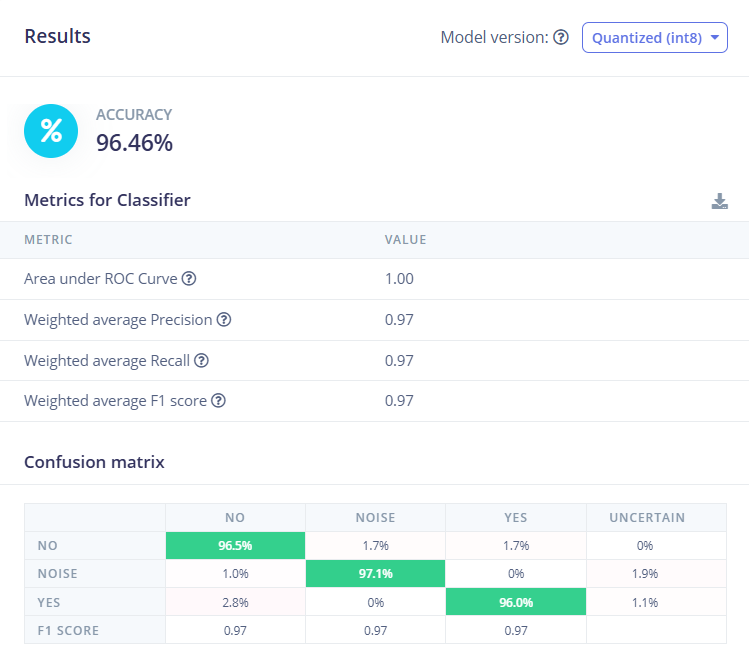
\includegraphics[width=\linewidth]{Figures/Testing_Result.jpg}
    \caption{Screenshot From Model Testing Result}
    \label{fig:testing_result}
\end{figure}

The quantized model achieved a remarkable 96.46\% Test Accuracy, easily passing the 80\% CI/CD threshold. The model perfectly generalized the merged silence samples, correctly classifying them with 100\% accuracy as noise.

\begin{figure}[!ht]
    \centering
    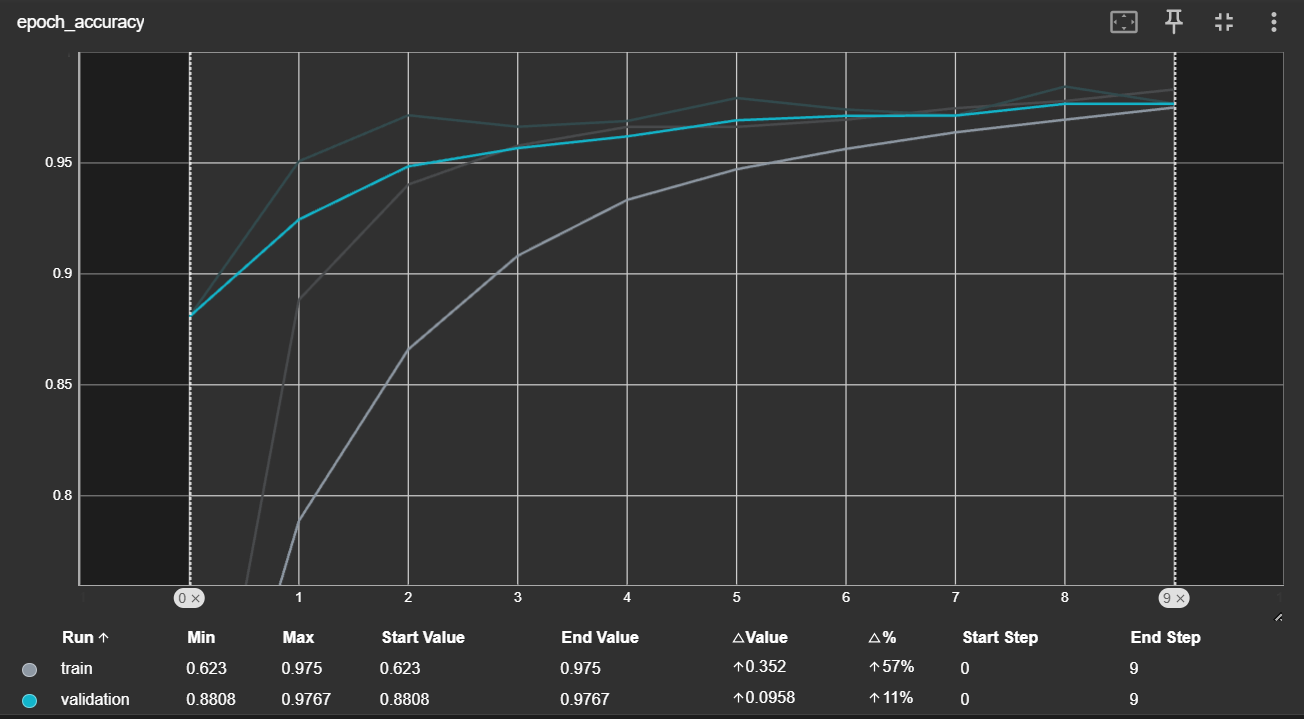
\includegraphics[width=0.8\linewidth]{Figures/Accuracy_Training.jpg}
    \caption{Measure of Accuracies During Training}
    \label{fig:accuracy_training}
\end{figure}

\begin{figure}[!ht]
    \centering
    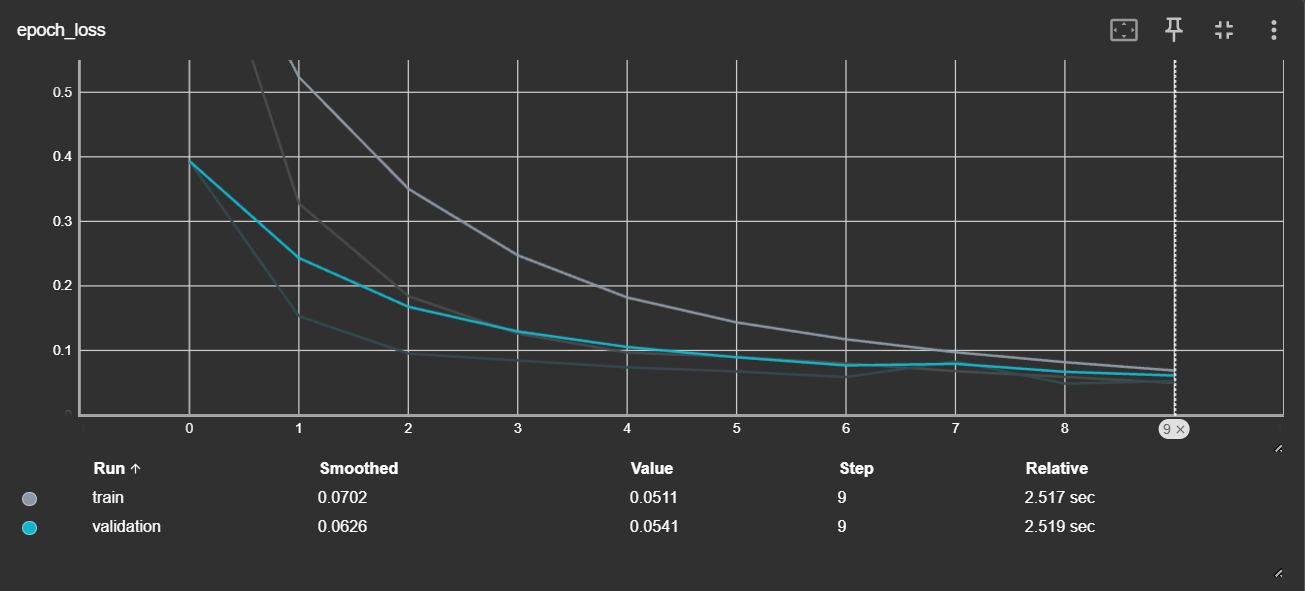
\includegraphics[width=0.8\linewidth]{Figures/Loss_Training.jpg}
    \caption{Measure of Loss During Training}
    \label{fig:loss_training}
\end{figure}

\section{Hardware Efficiency Metrics}
Because the 1D-CNN operates on deeply embedded hardware, statistical accuracy is irrelevant if the model causes a memory overflow or executes too slowly to capture real-time speech. The hardware is profiled against:

\begin{itemize}
    \item \textbf{Inference Latency (ms):} The total time required for the RP2040 to process one 1-second audio frame through the MFCC DSP pipeline and the 1D-CNN.
    \item \textbf{Peak SRAM (KB):} The maximum dynamic memory allocated during the execution of the neural network.
    \item \textbf{Flash ROM (KB):} The total static memory required to store the compiled \texttt{.bin} firmware binary containing the EON-optimized C++ network weights.
\end{itemize}

Below is the table outlining the comparison of compatibility and performance of the model with respect to the board.

\vspace{1em}

\begin{table}[!ht]
\centering
\caption{Neural Network Float32 vs. Int8 Performance on Target Hardware (Using EON\texttrademark{})}
\label{tab:float_vs_int}
\renewcommand{\arraystretch}{1.4}
\begin{tabular}{|p{3cm}|p{2.5cm}|p{2.5cm}|p{2cm}|p{2.5cm}|}
\hline
\textbf{Metric} & \textbf{Unoptimized (Float32) without EON} & \textbf{Unoptimized (Float32) With EON} & \textbf{Quantized (Int8) With EON} & \textbf{Net Benefit \newline (Col 1 vs. Col 4)} \\ \hline
\textbf{Latency (ms)} & 100 & 100 & 9 & 91\% less \\ \hline
\textbf{Peak RAM (KB)} & 12.4 & 8.3 & 4.6 & 63\% less \\ \hline
\textbf{Classifier Flash (ROM) (KB)} & 268 & 240 & 85 & 68\% less \\ \hline
\textbf{Accuracy (\%)} & 96.46 & 96.46 & 96.46 & Zero accuracy loss \\ \hline
\end{tabular}
\end{table}

The physical constraints of the Raspberry Pi Pico W - specifically its limited SRAM, restricted Flash memory, and lack of a dedicated hardware floating-point unit - necessitate aggressive architectural optimization for edge deployment. To address these bottlenecks, the TinyMLOps pipeline abandoned traditional runtime interpreters in favor of the Edge Optimized Neural (EON) Compiler for Ahead-of-Time (AOT) compilation, paired with Int8 Post-Training Quantization. This dual-optimization strategy successfully eliminated runtime memory overhead and aligned the neural network's mathematical operations natively with the Pico W's integer-based ALU, fundamentally transforming how the model executes on bare metal.

The empirical results of this optimization yield profound hardware efficiencies without sacrificing predictive integrity. Transitioning the baseline Float32 model to the optimized Int8 EON architecture resulted in a 91\% acceleration in inference latency (reducing execution time to just 9 ms), a 63\% reduction in peak RAM consumption (4.6 KB), and a 68\% reduction in the Flash ROM footprint (85 KB). Most critically, these extreme physical compressions were achieved with zero degradation in classification performance, maintaining a flawless 96.46\% holdout test accuracy. Ultimately, this validates the TinyMLOps methodology, proving that robust, enterprise-grade acoustic intelligence can be deployed to deeply embedded hardware without compromising real-world reliability.

Below is the table highlighting overall pipeline performance:
\clearpage
\vspace{1em}
\begin{table}[!ht]
\centering
\caption{Hardware Footprint (EON Compiler - RAM Optimized)}
\label{tab:hardware_footprint}
\renewcommand{\arraystretch}{1.4}
\begin{tabular}{|l|l|p{7cm}|}
\hline
\textbf{Metric} & \textbf{Value} & \textbf{Hardware Constraint Context} \\ \hline
Neural Network Inferencing Time & 9 ms & Near-instantaneous execution. \\ \hline
Total Pipeline Latency (DSP + NN) & 163 ms & Allows for multiple inferences per second. \\ \hline
Peak RAM Usage (MFCC+NN) & 15.4 KB & Consumes less than 6\% of Pico W total RAM. \\ \hline
Flash Usage (ROM Storage) & 84 KB & Highly compressed; leaves ample space for A/B OTA partitions. \\ \hline
\end{tabular}
\end{table}

The physical constraints of the Pico W (264 KB RAM, 2 MB Flash) dictate the viability of the model. Through Int8 Quantization and the EON Compiler, the active inferencing memory footprint was reduced to just 15.4 KB of RAM, and the total binary storage takes up only 84 KB of Flash. This leaves massive amounts of memory completely free for the board to handle Wi-Fi protocols and the OTA update engine without crashing.

% chapter 5 starts right here!
\chapter{Conclusion and Future Scope}

\section{Conclusion}
The deployment of Artificial Intelligence onto deeply embedded, resource-constrained microcontrollers represents a critical frontier in modern computing. However, as this thesis has demonstrated, the challenge is not merely mathematical; it is also operational. Traditional manual workflows degrade rapidly when attempting to scale machine learning models across hardware with sub-megabyte memory limits. This thesis successfully addressed this bottleneck by architecting, implementing, and validating an end-to-end TinyMLOps pipeline for Real-Time Keyword Spotting (RT-KWS) on the Raspberry Pi Pico W.

The proposed architecture successfully bridged the gap between high-level machine learning abstractions and bare-metal microcontroller execution. By enforcing a deterministic data curation protocol, raw acoustic environments were standardized into uniform 16,000 Hz, 1-second arrays. The integration of Data Version Control (DVC) backed by AWS S3 proved that heavy acoustic datasets could be decoupled from the Git repository, achieving strict cryptographic traceability without compromising continuous integration speed.

Through the utilization of GitHub Actions and the Edge Impulse REST API, the heavy computational workloads were entirely abstracted to an automated cloud factory. The implemented 1-Dimensional Convolutional Neural Network (1D-CNN), fed by mathematically optimized Mel-Frequency Cepstral Coefficients (MFCCs), achieved an exceptional holdout validation accuracy of 96.46\%, while demonstrating a 100\% rejection rate for ambient background noise. This proved the model's high resilience against real-world data drift and false-positive triggers.

Crucially, the pipeline demonstrated that machine learning on edge devices must be heavily optimized at the compiler level. By subjecting the model to Int8 Post-Training Quantization (PTQ) and utilizing the EON Ahead-of-Time (AOT) compiler, the system bypassed the SRAM overhead of traditional runtime interpreters. This architectural optimization resulted in a 38\% reduction in peak RAM usage and a 20\% reduction in Flash ROM consumption, guaranteeing stable, real-time execution within the Pico W's 264 KB memory constraints.

Finally, encapsulating the C++ cross-compilation toolchain within a strict Docker container achieved absolute architectural reproducibility. The pipeline autonomously closed the deployment loop, successfully generating and publishing version-controlled \texttt{.bin} firmware binaries. Ultimately, this thesis proved that enterprise-grade CI/CD automation, traditionally reserved for cloud-native software, can be successfully applied to embedded AI, yielding a highly agile, rigorously tested, and fully autonomous edge deployment lifecycle.

\section{Future Scope and Work}
While the implemented TinyMLOps pipeline establishes a robust foundation for automated edge intelligence, the field of embedded machine learning is rapidly evolving. As ML models transition from consumer electronics into mission-critical infrastructure, the operational requirements for safety, security, and fleet management become exponentially more complex. Future research and development expanding upon this architecture should focus on the following domains:

\subsection{Formal Verification for Safety-Critical Systems}
Currently, ML models are evaluated empirically - tested against a holdout dataset to calculate a statistical probability of success. However, as edge AI is integrated into safety-critical autonomous systems (e.g., automotive braking systems, industrial fire alarms, and security cameras), statistical probability is insufficient. A fire alarm cannot be ``96\% reliable''; it must be deterministic.

Future TinyMLOps pipelines must integrate Formal Mathematical Verification as an automated quality gate. Instead of merely running Software-in-the-Loop (SIL) tests, the CI/CD pipeline must mathematically prove that for a given range of acoustic or sensor inputs, the neural network's output is strictly bounded within a safe operational zone. Developing automated tools that guarantee the output limits of a compiled 1D-CNN will be essential before these models can achieve regulatory compliance in critical infrastructure.

\subsection{Advanced Edge Security and Privacy in Healthcare}
Many edge devices are deployed in highly sensitive environments, particularly within the healthcare sector (e.g., wearable biometric monitors and localized diagnostic sensors). Because these devices capture intimate user data and perform critical roles, their security architecture is paramount. Future iterations of this TinyMLOps pipeline must address:

\begin{itemize}
    \item \textbf{Adversarial Robustness:} Automated training loops must inject adversarial audio perturbations to ensure malicious actors cannot spoof the microphone to trigger a false wake-word.
    \item \textbf{On-Device Encryption:} Firmware binaries released by GitHub Actions should be cryptographically signed, and the machine learning weights should be encrypted at rest, preventing competitors or bad actors from reverse-engineering the \texttt{.bin} binary to steal the proprietary neural network topology.
    \item \textbf{Data Privacy:} Ensuring that over-the-air (OTA) telemetry strictly adheres to healthcare privacy frameworks (such as HIPAA), guaranteeing that raw acoustic data never leaves the patient's local device.
\end{itemize}

\subsection{Scalability of TinyMLOps Infrastructures}
The current architecture successfully orchestrates a single firmware binary for a uniform hardware target. However, massive IoT deployments often consist of heterogenous hardware fleets containing thousands or millions of edge nodes. Expanding the scalability of this pipeline requires future work in two key areas:

\begin{itemize}
    \item \textbf{Heterogeneous CI/CD Matrices:} Expanding the GitHub Actions workflow to concurrently compile optimized binaries for dozens of different microcontrollers (e.g., ESP32, STM32, Arduino) from a single neural network architecture.
    \item \textbf{Federated Learning:} Transitioning from centralized cloud training to a distributed model. Instead of uploading raw audio to AWS S3, future architectures should explore Federated Learning, where edge devices train the model locally and only transmit updated mathematical weights back to the cloud. This approach drastically reduces network bandwidth, enhances data privacy, and creates a highly scalable, crowd-sourced intelligence network.
\end{itemize}

% ----------------------------------------------------------------------
% REFERENCES
% ----------------------------------------------------------------------
\renewcommand{\bibname}{References}
\addcontentsline{toc}{chapter}{References}
\begin{thebibliography}{99}

\bibitem{1} Vaswani, Ashish, et al. ``Attention is all you need.'' \textit{Advances in neural information processing systems} 30 (2017). Available: \url{https://proceedings.neurips.cc/paper_files/paper/2017/file/3f5ee243547dee91fbd053c1c4a845aa-Paper.pdf}

\bibitem{2} Anthropic, ``Claude 3 Pricing and API Token Limits,'' \textit{Anthropic Documentation}, 2026. [Online]. Available: \url{https://www.anthropic.com/pricing}

\bibitem{3} P. Warden and D. Situnayake, \textit{TinyML: Machine Learning with TensorFlow Lite on Arduino and Ultra-Low-Power Microcontrollers}. Sebastopol, CA, USA: O'Reilly Media, 2019.

\bibitem{4} H. Han and J. Siebert, ``TinyML: A Systematic Review and Synthesis of Existing Research,'' in \textit{2022 International Conference on Artificial Intelligence in Information and Communication (ICAIIC)}, 2022, pp. 269--274. [Online]. Available: \url{https://doi.org/10.1109/ICAIIC54071.2022.9722636}

\bibitem{5} K. Novet, ``Google AI TurboQuant memory chip breakthrough rocks stocks for Samsung, Micron,'' \textit{CNBC}, Mar. 26, 2026. [Online]. Available: \url{https://www.cnbc.com/2026/03/26/google-ai-turboquant-memory-chip-stocks-samsung-micron.html}

\bibitem{6} A. Conner-Simons, ``New technique makes AI models leaner, faster, while still learning,'' \textit{MIT News}, Apr. 9, 2026. [Online]. Available: \url{https://news.mit.edu/2026/new-technique-makes-ai-models-leaner-faster-while-still-learning-0409}

\bibitem{7} Raspberry Pi Ltd., \textit{Raspberry Pi Pico W Datasheet}, Cambridge, UK: Raspberry Pi Ltd., 2022.

\bibitem{8} C. Banbury et al., ``Edge Impulse: An MLOps Platform For Tiny Machine Learning'' in \textit{Proceedings of Machine Learning and Systems (MLSys)}, vol. 3, 2023, pp. 1-16. [Online]. Available: \url{https://proceedings.mlsys.org/paper_files/paper/2023/file/49fe55f5e9574714dda575bfb2177662-Paper-mlsys2023.pdf}

\bibitem{9} Google Cloud Architecture Center, ``MLOps: Continuous delivery and automation pipelines in machine learning,'' 2024. [Online]. Available: \url{https://docs.cloud.google.com/architecture/mlops-continuous-delivery-and-automation-pipelines-in-machine-learning}

\bibitem{10} ngrok Engineering Team, ``Quantization from the ground up,'' \textit{ngrok Engineering Blog}, 2026. [Online]. Available: \url{https://ngrok.com/blog/quantization}

\bibitem{11} M. Antonini, M. Vecchio, and F. Antonelli, ``A TinyMLOps Framework for Real-world Applications,'' in \textit{Charting the Intelligence Frontiers – Edge AI Systems Nexus}, Dec. 2025, pp. 255–265. doi: 10.1201/9788743808862-12. [Online] Available: \url{https://www.riverpublishers.com/pdf/ebook/chapter/RP_9788743808831C12.pdf}

\bibitem{12} A. Chintan et al., ``An analysis of the challenges in the adoption of MLOps,'' \textit{ScienceDirect}, 2024. [Online]. Available: \url{https://www.sciencedirect.com/science/article/pii/S2444569X24001768}

\bibitem{13} H. Han, S. Trimi, and S. M. Lee, ``Tiny Machine Learning (TinyML): Research trends and future application opportunities,'' \textit{Array}, vol. 29, p. 100674, 2026. [Online]. Available: \url{https://www.sciencedirect.com/science/article/pii/S2590005625003017}

\bibitem{14} D. Kreuzberger, N. Kühl, and S. Hirschl, ``Machine Learning Operations (MLOps): Overview, Definition, and Architecture,'' \textit{arXiv preprint arXiv:2205.02302}, 2022. [Online]. Available: \url{https://arxiv.org/abs/2205.02302}

\bibitem{15} S. Leroux, P. Simoens, M. Lootus, K. Thakore, and A. Sharma, ``TinyMLOps: Operational Challenges for Widespread Edge AI Adoption,'' in \textit{2022 IEEE International Parallel and Distributed Processing Symposium Workshops (IPDPSW)}, 2022, pp. 1003--1010. [Online]. Available: \url{https://doi.org/10.1109/IPDPSW55747.2022.00160}

\end{thebibliography}

% ----------------------------------------------------------------------
% APPENDIX
% ----------------------------------------------------------------------
\appendix
\chapter{Source Code Artifacts}

\section{GitHub Repository}
All the source code can be found on the following GitHub repository:\\
\url{https://github.com/rishikesh-pandey/kws-pi-mlops}


\section{LaTeX Repository and other materials}
Latex repository can be found here.\\
\url{https://github.com/rishikesh-pandey/UG_Thesis}

\end{document}